% 09_sicurezza_incertezza.tex — Capitolo 9: Sicurezza e incertezza nell'IA.
% Documento didattico "Intelligenza artificiale nel progetto supervised_telemedicina".

\chapter{Sicurezza e incertezza nell'IA}\label{cap:sicurezza}

Nei capitoli~\ref{cap:distillazione} e~\ref{cap:valutazione} abbiamo visto
che l'MLP del progetto \progetto{} raggiunge un'accuracy di $0.9851$ sul
test congelato. È un buon numero, ma lascia 298 errori, concentrati vicino
ai confini di decisione. In questo capitolo affrontiamo la domanda che
ogni sistema clinico deve porsi: \emph{cosa succede quando il modello
sbaglia?} La risposta del progetto è una architettura a tre livelli:
un safety gate deterministico che ha precedenza assoluta, una misura
esplicita dell'incertezza e un fallback testuale quando il modello è
troppo incerto.

\section{Perché un modello da solo non basta in clinica}\label{sec:perche-modello-non-basta}

Un modello di machine learning è un approssimatore: per costruzione sbaglia
su una frazione dei casi. In un'applicazione di raccomandazione di film un
errore è innocuo; in telemedicina un errore su un caso critico può avere
conseguenze serie. Un paziente a rischio \classe{alto} scambiato per
\classe{basso} è un paziente che non riceve l'attenzione che merita.

Per questo il progetto parte da un principio progettuale esplicito, ripreso
dall'architettura del safety gate (capitolo~\ref{cap:teacher}): l'IA deve
essere un \emph{supporto}, non un oracolo. Il modello può contribuire a
rendere le decisioni più fluide e informate, ma non può essere l'ultima
parola su un caso che le regole cliniche giudicano critico. Questo si
traduce in codice: le regole deterministiche hanno \emph{precedenza
assoluta} sul modello.

\section{Il safety gate deterministico}\label{sec:safety-gate}

La figura~\ref{fig:diagramma-flusso-gate} mostra il flusso decisionale a
runtime: i parametri vitali entrano nel safety gate rule-based; se il caso
è critico, la risposta viene emessa subito dal gate (con notifica); altrimenti
il controllo passa al MLP, che produce una classe e una confidenza.

\begin{figure}[htbp]
  \centering
  % diagramma_flusso_gate.tex — diagramma TikZ (incluso dai capitoli).
\begin{tikzpicture}[
    nodo/.style={draw, rounded corners=2pt, minimum height=0.9cm, align=center, font=\small},
    decisione/.style={diamond, draw, aspect=2.2, align=center, font=\small, inner sep=1pt},
    freccia/.style={-{Stealth[length=2.5mm]}, thick},
  ]
  \node[nodo, fill=blue!10] (par) at (0,0) {Parametri vitali\\6 feature};
  \node[decisione, fill=yellow!20] (gate) at (3.2,0) {Safety gate\\rule-based};
  \node[nodo, fill=red!15] (crit) at (6.8,1.6) {Caso critico\\GATE + NOTIFICA};
  \node[nodo, fill=green!15] (mlp) at (6.8,-1.6) {MLP (softmax)};
  \node[decisione, fill=yellow!20] (soglia) at (10.2,-1.6) {Confidenza\\$< 0.6$?};
  \node[nodo, fill=orange!15] (fallback) at (13.6,-2.9) {Fallback\\rule-based};
  \node[nodo, fill=green!15] (classe) at (13.6,-0.3) {Classe MLP\\+ metadati};
  \draw[freccia] (par) -- (gate);
  \draw[freccia] (gate) -- node[above, font=\scriptsize] {critico} (crit);
  \draw[freccia] (gate) -- node[below, font=\scriptsize] {non critico} (mlp);
  \draw[freccia] (mlp) -- (soglia);
  \draw[freccia] (soglia) -- node[right, font=\scriptsize] {sì} (fallback);
  \draw[freccia] (soglia) -- node[above, font=\scriptsize] {no} (classe);
\end{tikzpicture}

  \caption{Il flusso decisionale di \codice{SupervisedAgent.predict}: il
  safety gate rule-based ha precedenza assoluta; l'MLP viene consultato solo
  sui casi non critici e la sua risposta è filtrata dalla soglia di
  incertezza (0.6).}
  \label{fig:diagramma-flusso-gate}
\end{figure}

Il codice reale in \file{src/telemedicina\_supervised/agents/supervised\_agent.py}
è esplicito. Le prime righe di \codice{predict} applicano il gate prima di
qualsiasi inferenza:

\begin{lstlisting}[caption={Il safety gate con precedenza assoluta in \codice{SupervisedAgent.predict} (\file{supervised\_agent.py}).}]
def predict(self, parametri: Any) -> AgentOutcome:
    dettagli = analizza(parametri)
    if not dettagli["valido"]:
        return self._base(dettagli, errore=True)

    base = self._base(dettagli)
    # Critical and pattern-dangerous outcomes are returned byte-for-byte
    # at the established fields; only additive metadata is populated.
    if dettagli["classe"] == "alto":
        return base

    modello, motivo = self._carica()
    if modello is None:
        base.fallback = True
        base.motivo_fallback = motivo
        return base
\end{lstlisting}

La riga chiave è \codice{if dettagli["classe"] == "alto": return base}:
se le regole giudicano il caso critico, l'MLP \emph{non viene mai
consultato}. Il caso non può essere declassato: la risposta è quella del
safety gate, con motivo esplicito \codice{"safety gate: classe critica,
MLP bypassato"}. La funzione \codice{analizza} usata qui è la stessa del
teacher (capitolo~\ref{cap:teacher}), quindi gate a runtime e label offline
non possono divergere.

\begin{esempio}{Un caso critico non passa dall'MLP}
Con i parametri (185, 110, 80, 36.8, 98, 95) — crisi ipertensiva — le
regole rispondono \classe{alto}. Il gate intercetta il caso prima dell'MLP:
il modello non viene nemmeno caricato. Non c'è alcun modo, nel codice, che
un caso \classe{alto} venga declassato a \classe{medio} o \classe{basso}:
è una proprietà \emph{per costruzione}, non un comportamento statistico.
\end{esempio}

\section{L'incertezza del modello}\label{sec:incertezza-modello}

Quando il caso non è critico, il controllo passa al MLP. La rete produce
una distribuzione softmax sulle tre classi (capitolo~\ref{cap:reti}), e il
progetto usa la \emph{confidenza} — la probabilità massima — come misura
di incertezza. La figura~\ref{fig:istogramma-confidenze} mostra la
distribuzione della confidenza sul test congelato, con la soglia di
incertezza evidenziata.

\begin{figure}[htbp]
  \centering
  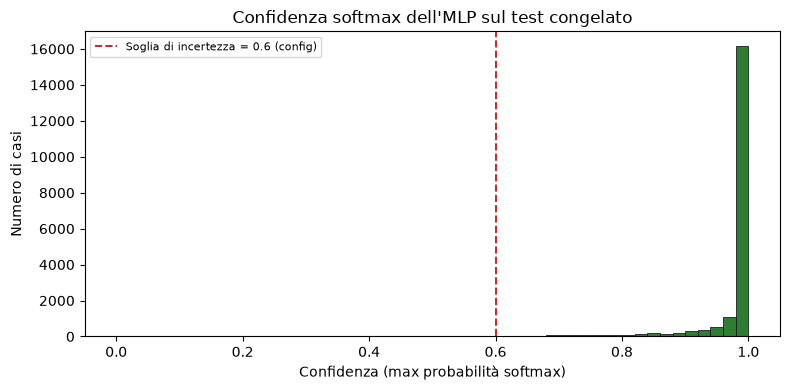
\includegraphics[width=0.85\textwidth]{figure/generate/istogramma_confidenze.png}
  \caption{Istogramma della confidenza softmax del MLP sul test congelato.
  La linea verticale marca la soglia di incertezza (0.6): a sinistra i casi
  in cui il modello è troppo incerto per decidere da solo.}
  \label{fig:istogramma-confidenze}
\end{figure}

L'istogramma ha due code ben separate: una massa di casi in cui il modello è
molto sicuro (confidenza vicina a 1) e una coda di casi incerti sotto la
soglia. La soglia vive in \file{src/telemedicina\_supervised/config.py}
come \codice{SOGLIA\_INCERTEZZA = 0.6}, in modo che sia un parametro
esplicito, modificabile senza toccare il codice dell'agente.

Una nota onesta: la confidenza softmax \emph{non} è una probabilità
calibrata. Il valore $0.6$ non significa ``il 60\% dei casi con questa
confidenza è corretto'': la softmax misura la \emph{competizione relativa}
tra classi, non la correttezza assoluta. È comunque una \emph{ordinata}
misura di incertezza: in media, più la confidenza è bassa, più il modello
sbaglia. Il progetto la usa come segnale per il fallback, non come
garanzia statistica.

\section{Il fallback}\label{sec:fallback}

Se la confidenza è sotto la soglia, il modello non viene ignorato in
silenzio: il progetto ripiega sulle \emph{regole testuali} con un motivo
esplicito. Il codice reale:

\begin{lstlisting}[caption={Il fallback per confidenza sotto la soglia in \codice{SupervisedAgent.predict}.}]
        confidenza = float(probabilita_array[indice_mlp])
        base.modello_usato = True
        base.classe_mlp = classe_mlp
        base.classe_regola = base.classe
        base.confidenza = confidenza
        base.probabilita = probabilita
        base.override_sicurezza = (CLASSI.index(base.classe) > indice_mlp)
        if confidenza < SOGLIA_INCERTEZZA:
            base.fallback = True
            base.motivo_fallback = "confidenza sotto la soglia di incertezza"
            return base
\end{lstlisting}

Due osservazioni sul codice. Primo, \codice{base} contiene già la classe
rule-based (calcolata da \codice{analizza}): quando il modello è troppo
incerto, il sistema restituisce la decisione del safety gate, arricchita
dai metadati \codice{fallback=True} e \codice{motivo\_fallback}. Secondo,
il campo \codice{override\_sicurezza} segnala i casi in cui la regola è più
conservativa dell'MLP (classe di regola con indice maggiore): è una
traccia esplicita per chi legge l'esito che, dove le regole e il modello
non concordano, la sicurezza ha la precedenza.

\section{Notifiche e tracciamento}\label{sec:notifiche-tracciamento}

Un sistema clinico non deve solo rispondere: deve \emph{lasciare traccia}.
In \progetto{} ogni analisi viene persistita in un database SQLite
(\file{data/analisi.db}) con due tabelle, definite in
\file{src/telemedicina\_supervised/database/analisi\_db.py}:

\begin{itemize}
  \item \codice{analisi}: una riga per analisi, con timestamp, classe,
        probabilità, messaggio e i \emph{metadati} dell'esito;
  \item \codice{notifiche}: una riga per ogni caso critico, con timestamp,
        classe e messaggio.
\end{itemize}

I casi critici (classe \classe{alto}, o input non validi) generano una
notifica: il servizio \file{services/notifications.py} la scrive nel
database e su \codice{stderr}. L'oggetto \codice{AgentOutcome} trasporta i
metadati: \codice{modello\_usato}, \codice{classe\_mlp},
\codice{classe\_regola}, \codice{confidenza}, \codice{fallback},
\codice{motivo\_fallback}, \codice{override\_sicurezza}. Così ogni analisi
può essere ripercorsa: sappiamo sempre \emph{chi} ha deciso (regole o
MLP), \emph{con quanta fiducia} e \emph{perché} è stato attivato il
fallback.

\section{Richiamo 1.0 per costruzione}\label{sec:richiamo-per-costruzione}

Nel capitolo~\ref{cap:valutazione} abbiamo visto che l'MLP \emph{da solo}
ha recall $0.9958$ sul \classe{alto}: 30 casi critici su 7100 sfuggono alla
rete. Se il sistema fosse solo l'MLP, quei 30 pazienti sarebbero
classificati \classe{medio}: un rischio clinico reale.

Con il safety gate, però, la storia cambia radicalmente. Il gate intercetta
\emph{tutti} i casi \classe{alto} prima dell'MLP: il recall del sistema
completo sui casi critici è \textbf{1.0 per costruzione}, non per fortuna.
Non è un risultato misurato su un test: è una garanzia strutturale del
codice. I 30 mancati del modello non esistono più nel sistema, perché il
modello non vede mai quei casi.

\begin{esempio}{Modello vs sistema}
La metrica del capitolo~\ref{cap:valutazione} misura il \emph{modello}
(MLP isolato); il safety gate misura il \emph{sistema} (gate + MLP +
fallback). La distinzione è fondamentale: un'architettura di sicurezza
non migliora il modello, \emph{contiene} i suoi errori. Il costo è la
precisione: alcuni casi \classe{medio} che l'MLP avrebbe azzeccato vengono
gestiti dal gate. È uno scambio accettato e documentato dal progetto: in
clinica, il falso allarme costa meno di un caso critico mancato.
\end{esempio}

Questo è il senso profondo dell'architettura: il modello serve dove le
regole sono ambigue, il gate garantisce dove le regole sono nette, e il
fallback ammette l'incertezza dove nemmeno il modello sa decidere. La
sicurezza non è un ripensamento: è il vincolo che ha dato forma al codice
fin dal primo capitolo.
